%%%%%%%%%%%%%%%%%%%%%%%%%%%%%%%%%%%%%%%%%
% Intermediate report
% Version 1.0 (10/16/13)
%
% This template has been downloaded from:
% http://www.LaTeXTemplates.com
%
% Original Authors:
% Darren Chu
% Todd Detweiler
% Cody Kagawa
% Lauren Swanson
% Dogni Wang
%
%%%%%%%%%%%%%%%%%%%%%%%%%%%%%%%%%%%%%%%%%

%----------------------------------------------------------------------------------------
%	PACKAGES AND OTHER DOCUMENT CONFIGURATIONS
%----------------------------------------------------------------------------------------

\documentclass[a4paper, 11pt]{article} % Font size (can be 10pt, 11pt or 12pt) and paper size (remove a4paper for US letter paper)
\usepackage[utf8]{inputenc}
\usepackage[protrusion=true,expansion=true]{microtype} % Better typography
\usepackage{graphicx} % Required for including pictures
\usepackage{wrapfig} % Allows in-line images
\usepackage{pdfpages}

\usepackage{mathpazo} % Use the Palatino font
\usepackage[T1]{fontenc} % Required for accented characters
\linespread{1.05} % Change line spacing here, Palatino benefits from a slight increase by default

\DeclareGraphicsExtensions{.pdf,.png,.jpg}


\makeatletter
\renewcommand\@biblabel[1]{\textbf{#1.}} % Change the square brackets for each bibliography item from '[1]' to '1.'
\renewcommand{\@listI}{\itemsep=0pt} % Reduce the space between items in the itemize and enumerate environments and the bibliography

\renewcommand{\maketitle}{ % Customize the title - do not edit title and author name here, see the TITLE block below
\begin{flushright} % Right align
{\LARGE\@title} % Increase the font size of the title

\vspace{50pt} % Some vertical space between the title and author name

{\large\@author} % Author name
\\\@date % Date

\vspace{40pt} % Some vertical space between the author block and abstract
\end{flushright}
}

%----------------------------------------------------------------------------------------
%	TITLE
%----------------------------------------------------------------------------------------

\title{\textbf{Final Report for Object Creator Team}} 

\author{\textsc{Darren Chu\\Todd Detweiler\\Cody Kagawa\\Lauren Swanson\\Dongni Wang} % Author
\\{\textit{University of Puget Sound}}} % Institution

\date{\today} % Date

%----------------------------------------------------------------------------------------



\begin{document}

\maketitle % Print the title section
\newpage

\section*{Table of Contents}
\section{\emph{Object Creator Project Summary}}
\section{\emph{Development Procedures}}
\section{\emph{Requirement Evaluations}}
\section{\emph{System Design} \& \emph{Architecture}}
\section{\emph{Individual Reflections}}
\section{\emph{Glossary and References}}   

\newpage
%----------------------------------------------------------------------------------------
%	ESSAY BODY
%----------------------------------------------------------------------------------------

\section*{Project Summary}

Our module was the object creation component of a greater project, Edith. Edith is an educational programming system aimed at teaching younger students to code through a graphical drag and drop interface. The user is able to select blocks that represent common pieces found in code, such as loops, if-statements, etc., to create stories with characters they have created. These characters, or sprites, are created in our module, the Object Creator. This module was developed to enable the user to create sprites and other story elements. The user is able to create the objects through painting, manipulating geometric primitives, or importing their own images from other sources. Users are able to easily switch between the Object Creator and the Story Creator, where the animations are assembled. Here, in the Story Creator, the user is able to code movements for their new objects and add them to the overall story.

Our module opens as a separate window to the Story Creator and displays a canvas accompanied by object creations tools.  After the user has added their object to the canvas, they have the ability to resize and rotate the object to obtain their ideal character or story component. The user is also allowed to add layers to their object as to provide more pieces that can be animated individually in their story. When the object is complete, the layers of the canvas are exported together, under one name, as a JavaScript object to the Sharing Framework. Here, the created object is accessible to the other system modules. This allows the user to move to the Story Creator and upload their new object onto the Visual Editor canvas. 

%------------------------------------------------

\section*{Development Procedures}

To create our model, we originally implemented an Abstract Factory software design pattern. We chose this design pattern because our module is based on creating objects but creates those objects in different fashions. The user can either import an image, draw, or build a character out of primitive geometric shapes. These are then compiled into an image grouping composed of various shape objects. An Abstract Factory design pattern is defined as one which groups individual factories that have a common theme. Because all of our classes dealt with the larger picture of creating an image and forming an object but do it in different forms, we believed that an Abstract Factory design pattern best fulfilled the architecture we have laid out. However, the design pattern and requirements documents were not particularly useful as both became obsolete when the structure of our outputs was changed around integration 2, and the work to lay the program out again following this would have taken more time than it saved.

        	In terms of our specific approach to development, the underlying structure of our project was changed several times in order to accommodate new requirements, causing us to forego some of the planning and layout stages of production. Most of the decisions to implement changes were agreed upon informally as a group, followed by basic implementation by whoever suggested the change. Methods and design changes were delegated individually amongst ourselves and addressed on a case by case basis.
        	Our first priority was to produce a functional canvas with some means of producing shapes. We started with the basic html canvas and produced the circle, line, rectangle, and free draw functions. These were heavily modified following the decision to instead use the kinetic canvas, which provided us with built-in layering and drag-and-drop functionality. Once this was completed, we began work on image importing and layering, as well as color options. After those were came saving and deleting objects and layers, and finally scaling and rotation. A help button, background changes, and other formatting were added to improve usability of the program.
        	
        	The majority of the testing done on our project was performed individually and manually, though Qunit was used to identify the root of certain problems. Manual testing proved easier as proper program function produced visible results. Beyond that the program was not extensively tested, and communication with other modules was only occasionally tested. Testing within the code was difficult as the program did not produce an easily analyzable output.
        	
        	Cody was mostly involved with the delete shape and free draw methods, mostly as a result of complications with them following the change of canvas. He was also responsible for the abstract of the use cases, and the UML diagram in the requirements document. Todd contributed to the lower levels of the object creation program. This including creating the layers of a canvas, keeping track of those layers, implementing layer commands (delete layer, create layer, clear layer), saving layers into one javascript array with names associated to each layer, exporting those layers through Ajax into the saving framework, and then working with saving and sharing group to make sure the objects could correctly be loaded into the main project and used. Lauren took care of our user interface, helping it look nice and providing a help page to instruct users on the functions of our program. She also helped communicate with other teams to make sure they were getting what they needed and things were working. Dongni took care of a lot of the graphical functions and appearance of our application. She worked on many graphical abilities such as rotate, re-size, and importing images. She also tidied up the page changing the inputing method of variables and making the page a lot more neat and compact. Darren completed System architecture section of this paper.


%------------------------------------------------

\section*{Requirements Evaluation}

\\
\textbf {Functional Requirement:} \\*

1.	Create Object—object creator would allow the users to create sprite (by drawing/importing image), specify identifier for different parts, save and send converted JSON file to story editor.

This requirement is mostly like a wrapper requirement for the whole object creation module. It is met and only the order of the flows of events has been altered. Although this requirement is not very detailed, it is still a helpful one. We were able to test the integration result of different components based on this requirement because it covers the flow of events from the very start (click “create object” from the main page) to the end of object creation task (objects and identifiers has been created and saved for other modules to use). We know our module is fully functional if the create object requirement is met.\\

2.	Create Sprite—users would be able to create sprite on canvas using multiple drawing method. 

The requirement is met and again some events have been slightly altered. Instead of creating new canvas and window every time, now we just need to create a layer in the current window as KineticJS canvas has built in layers and each layer could be saved separately. Moreover, since there are no more pop-up windows, events for “storing canvas data” and “saving canvas data” are no longer present in the final implementation. Instead, we created a separate “save” button to save and send the information of multiple layers. This requirement is not as effective because it has been changed a lot after we implemented Kinetic Canvas. \\

3.	Specify object’s names—editors could specify the names of the object, and those names with associative sprite parts would be saved and sent to story editor for further use.

This requirement is met and the flow of events has been simplified as we implemented the Kinetic Canvas, which has built-in layers and stages. Currently each layer represents a part of the created sprite and could be exported as a separate object with a unique name. Besides, users need to specify the name of layers as they create the layers. This requirement is not very helpful. None of the user case events are preserved because we underestimated the complexity of specifying objects’ names after creating objects.\\

4.	Object Manipulation—editors can manipulate the objects. The editor can access the object manipulations menu and change the object with the specific methods in the menu.

This requirement is met while we didn’t create a menu for manipulation methods. In our module, moving objects is done by simply “drag-and-drop”. And for rotating, scaling, and deleting objects, we created radio buttons so that it is easier to use. The requirement was helpful and our final module functions as described in user case events except for the menu part.\\


5.	Importing image—importers would be able to add local image to canvas.

This requirement is met and was very helpful during implementation of this function. The flow of events are properly wrote and with enough details.
\\

\textbf {Non-functional Requirement:} \\*

1. 	Availability:

- The Object-creator module would be available whenever the users log into systems with PC or Macintosh platforms.
-The object-creator module should not fail for most of cases.

This requirement is partially met. The object-creator module would be available whenever the users log into systems given that the server is already connected. The module shall not fail for most of cases based on individual tests.\\

2.	Usability:
-The users are not expected to have any knowledge of or previous experience programming.
-For users with basic computer operation ability, the average time of learning the facilities of the module independently should be no more than one hour.
Ten minutes of training before independent use is possible.
-On average, the users with previous experience using graphics editing pro-
gram may make errors no more than 5 times per hour. The new users may
make more errors while learning, but should be able to be skilled users in
one hour with informative error messages and well-formed graphical user in-
terfaces.

This requirement is met. Our module has provided the help button with detailed guidelines. Input errors would be caught with informative alert message so that users could recover from error. For irrevocable commands like “deleting shape”, confirm boxes would prevent unintended operations of users.\\

3. 	Documentation:
-The documentation of object-creator module should be fully understandable to the animation module group.

This requirement is partially met. The final module was not fully documented as it has been revised many times. Instead, we sent group members to directly talk to animation module group and make sure they understand our code.\\






%------------------------------------------------

\section*{System Design and Architecture}
High-Level Walk through:\\

The Object Creator module of Edith is responsible for creating and design an object to be uploaded on to the main Edith canvas. In order for this to be done, we created a separate pop-up window from the original home page to the object creation canvas. In this page, the user will receive a canvas to work on. On this canvas, the user creates the characters or sprites. The user is able to create and manipulate the objects through, free draw, creating primitive geometric shapes, or import their own images from other sources. Users will be able to switch between the Object Creator and the Story Creator by exporting the image to the Story Creator’s object viewer in the homepage. 

On our separate window, we display a canvas and several object creation tools that can be utilized by buttons. The separate window design has a help pop-up button that will display detailed instructions that will help the user utilize the canvas. Below the canvas is the object creation too; buttons. Each of the buttons utilizes mouselisteners to draw the shapes and manipulate objects on a specific layer. When the object has been completely finished, the user will be able to save the objects to individual layers. Once the user has saved their objects and are complete, the layers of the canvas will be exported together under a single name. The exported object will be exported as a JavaScript object and will then be handled by the Sharing Framework.  Once exported, the other system’s modules can handle the object. 


Low-Level Walkthrough:\\

The object creator module is build of three major scripts, ObjectCreation.html, ObjectCreationStyleSheet.css, and the helpPopUp.html. The script in our module is the ObjectCreation.html. The main object creator display window is made up of the objectcreation.html, which displays the canvas, buttons and display window, and supplies the functionality.  The ObjectCreationStyleSheet.css is a stylesheet that was implemented to give the main object creator display window a border and a background. Finally, the pop-up window code is defined in the helpPopUp.html. This walkthrough will first explain the smaller components, ObjectCreationStyleSheet.css, and helpPopUp.html, before addressing the ObjectCreation.html.

ObjectCreationStyleSheet.css:\\

The ObjectCreationStyleSheet.css implements a stylistic background to our Object Creator canvas. The CSS implements a grey colored background, which allows the user to distinguish the canvas from the default white background. The CSS is also implemented in the helpPopUp.html to also give the pop-up the similar grey background color. 

helpPopUp.html:\\

The helpPopUp.html provides the pop-up window for the user. The pop-up window is used to relay instructions on how to create an object. The instructions include adding shapes, uploading an image, free draw, manipulating objects, using different layers and saving objects. Inside the script, the instructions are written within the code. The code then displays and separates each of the sections depending on their category and instructional heading.

ObjectCreation.html:\\

ObjectCreation.html is our main script in the Object Creator module. The code presents the majority of the Object Creator module’s functionality. It provides the user with a canvas, and object creation tools. The ObjectCreation.html utilizes multiple imports such as the KineticJS canvas library, JQuery and the ObjectCreationStyleSheet.css. The code sets up a kinetic js canvas for object creation, uploading images, and saving an array of JavaScript objects on a kinetic js layer.   

For our Object Creator window, we wanted the canvas, the heading, and the object creation tools in the center of the window. Therefore, we set all of our script positioned at the center. We first created the header, “Make a New Object.” and the Need Help? button above the canvas. The Need Help? button is linked to the helpPopUp.html and if clicked, will display the helpPopUp.html window.   

We started by creating a separate div section under the id of container. The container script starts by instantiating the layerArray. The layerArray will be used to store the kinetic js layer and all of its sprites. We then set the kinetic js canvas and its width and height variables. Next, the script sets up the kinetic js layer and then adds the kinetic later to the kinetic canvas. Finally, the container sets up the variables that will be implemented and manipulated throughout the script.

The next div section is labeled drawing. This part of the script consists of the bulk of our functions. The functions consist of:\\

1.	function changePriority(layer) allows the user to change the priority of which layer the user wants to draw on. This will allow the user to prioritize which layer they would want in front and add them to the layerArray. The layerArray will store the currently opened project and the selected layer due to their priorities.\\

2.	function scaleO(obj) allows the user to manipulate the size of the object. After selecting an object, the function will then use the object as its parameter. The scale function will prompt a user for an integer value input. The scale function will take in the user’s input and scale the object according to the numerical value. Once the object has been scaled, the newly manipulated object will be drawn onto the canvas. If the user inputs a non-integer value, the object will not change. Instead, an alert will prompt the user to use only integer inputs.\\


3.	function rotateO(obj) allows the user to rotate the object. After selecting an object, the function will then use the object as its parameter. The rotate function will prompt a user for an integer value. The function then takes in the user’s input and will the object according to the numerical value based on degrees. Once the object has been rotated, the newly manipulated object will be drawn onto the canvas.\\

4.	function drawLine(), function drawRec(), function drawCircle() allows the user to draw primitive shapes. Based on the prompted integer value, the canvas will draw the respective kinetic shape onto the current layer. The layer is then added and displayed onto the canvas.\\


5.	function clearCanvas() allows the user to clear the layer of the canvas. The function calls the kinetic layer’s built in method destroyChildren(). This method deletes the data from the layer and wipes the canvas.\\

6.	function uploadImage(e) is used to upload images onto the canvas. The upload image function will open a separate window that displays the user’s computer and files. The user can then select image and then display the image on the canvas. The image is automatically scaled down to a 100-pixel by 100-pixel image in order to fit on the canvas. \\


7.	function saveObject() is a function that will allow the user to save objects into the savedObjects array. The function will prompt the user to input a name. Once the name has been inputted, the layer will be saved under that name and push the layer and image name into the savedObjects array. Once the image has been successfully saved, an alert will appear notifying the user that the layer has been saved. If the user does not input a name, the function will send another alert prompting for a name. \\

8.	function displayImage() In this function, the user will be allowed to load an image onto the canvas, specifically load a layer onto the canvas. In this method the user will be prompt to enter a name of the image they want to load. Once the name has been inputted, the function will search through the savedObjects array and find the file with the same name. The array will then extract the file source data and display it onto the canvas. However, if the image was not found, it will alert the user that the specific image does not exist.\\

9.	function exporting() is a function that will send our objects and images to the other modules. The function prompts the user for a name. The function stores our ObjectArray under then name of the prompted name input. The kinetic ObjectArray is then stored within a sending array that will be sent to the story creator and visual editor to access and manipulate.\\

10.	function addLayer() allows the user to add another layer to the canvas. The function will prompt the user to input a name for the new layer. Once the name has been input, the layer will be stored under this name and then created. The newly created layer will then be put at the top of the layerArray. Once at the top of the layerArray, new all drawings and object creations will be added to this newly added array because the priority of the layer is set at the top.  \\

11.	function move(evt) takes in the user’s mouse events and allows the user to move the image around on the canvas. By taking in a mouselistener, if the mouse button is pressed down and the object is selected, by moving the mouse, the mouselistener will move the shape according to how the user moves their mouse. \\

12.	function drawfinal() is the function that allows us to free draw. The free draw function takes in a kinetic line draw function. However, the points at which the kinetic line draw function draws the shape depends on the path of the mouselistener. Since the path is based on the mouselistener, we are allowed to draw shapes freely depending on how the user moves their mouse. We also have the mousedownB set to false, but will switch to true when the left mouse button is pressed down. When the mousedownB is true the user can free draw, but if the left mouse button is not pressed down, the mousedownB is set to false, the user cannot free draw. \\

13.	function removeShape(shape) is a simple function that allows us to delete shapes from the layer. The method takes in a specific shape and deletes them from the layer. Once the layer has deleted the shape, the later is added to the canvas. \\

14.	function deleteLayer() is a function that allows the user to completely delete a layer from the layerArray. The layer calls the kinetic layer function destroy(). The destroy() function completely removes the layer. \\

15.	function saveAllObject() is the last function in the draw dive tag. This method stores all of the objects within the layer into an empty slot of the savedObjects. The layer is pushed into the savedObjects array with the image data and the image name as the parameters. Once the layer has been saved, an alert will tell the user that they have successfully saved the object.\\

The next div tag section is the radio section. This section displays the tab bar at the bottom of our Object Creation window. The main function within the radio dive section is the wipeListeners() function.

function wipeListeners() is the main function that receives the mouseListener inputs in relation to the tab bar. Depending on what object creation tool that the user wants to use from the tab bar, the wipeListener uses booleans as a switch. By setting these booleans to true, the user will be able to use different functions. The booleans are:\\

1.	destoryRB – When this variable is set to true, the user will be able to delete an object. \\

2.	rotate – When this variable is set to true, the user will be able to rotate the object. \\

3.	scale – When this variable is set to true, the user will be able to scale the object. \\

Each of these tabs on the tab bar are connected to the choice1(), choice 2(), choice3(), choice4() and choice5() functions. Each of these choices is labeled based on their functional use in the tab. \\

1.	function choice 1() does not have any functions besides using calling the mouselistener, Choice1() is labeled under the none tab.\\

2.	function choice2() allows the user to delete an object by setting the destroyRB variable to true. Choice2() is labeled under the delete shape tab.\\

3.	function choice3() allows the user to free draw by calling the drawFinal function. The drawFinal function is our function for free drawing and by pairing the mouselistener with the drawFinal function, the user can free draw. Choice3() is labeled under the free draw tab.\\

4.	function choice4() allows the user to rotate the object by setting the rotate variable to true. Choice4() is labeled under the rotate tab.\\

5.	function choice5() allows the user to scale the object by setting the scale variable to true. Choice5() is labeled under the scale tab.\\

The last function in the script is the helpUp(url) function. The function links the Need Help? button to the helpPopUp.html. When the user presses the button, the helpPopUp.html will pop up in a new window. With the focus() function, the pop up window will appear in front of the canvas because the focus priority will at front.


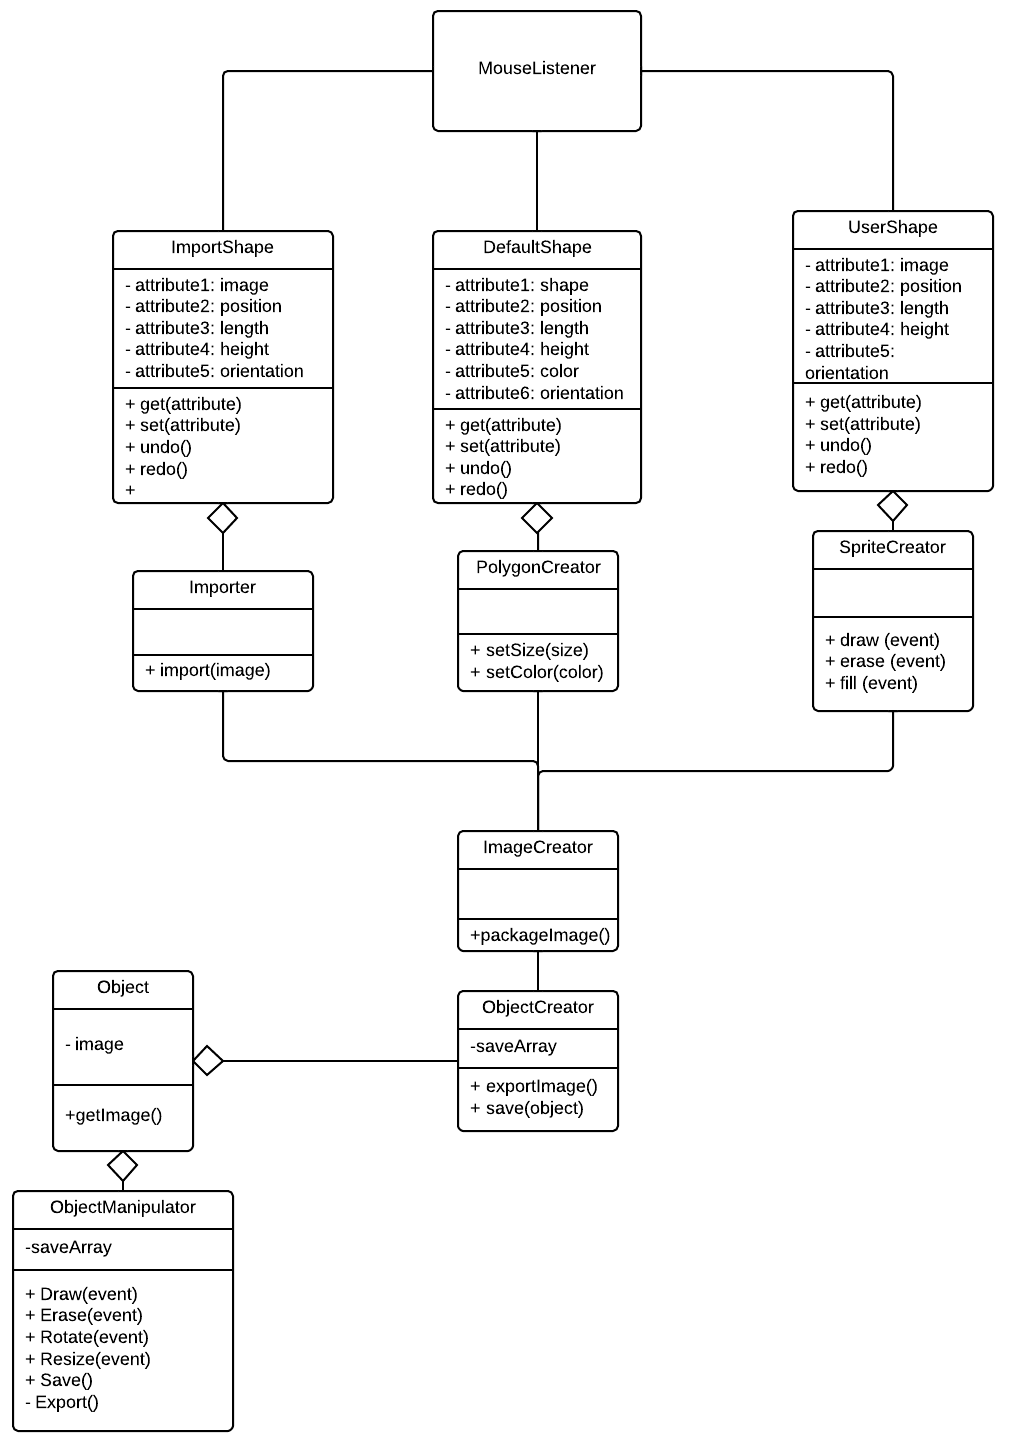
\includegraphics[scale=0.52]{ClassDiagramObjectModule}\\
A UML class diagram is given to represent the architecture of our system.\\

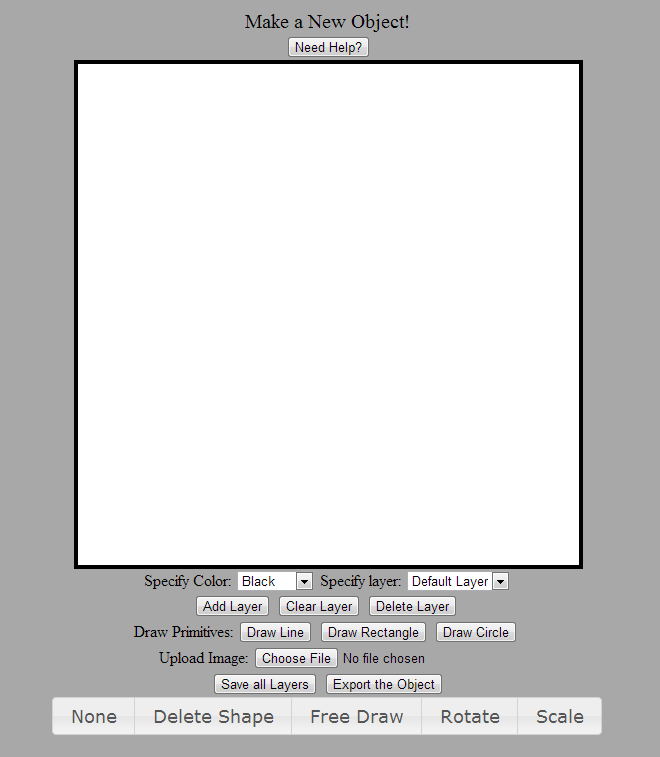
\includegraphics[scale=.7]{mainpage}\\
A screenshot of the user interface for the object creator page is displayed above.\\
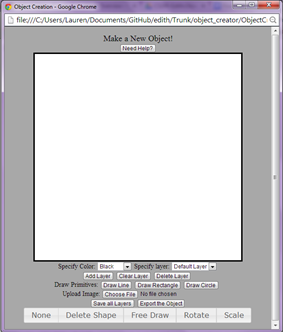
\includegraphics[scale=.8]{helppage}\\
A screenshot of the help page for our online application is displayed above.

%------------------------------------------------

\section*{Individual Reflections}

\subsection{Lauren}
We began our project by collaborating on our Requirement Specifications and I really liked how our group worked together, even during this early assignment. We all contributed to a Google Document with our parts of the paper and met multiple times to review each other’s work. I think it worked really well was very happy with our communication on the assignment. This translated to our Integration checkpoints, when we began working on our module. I really liked how we were able to communicate and find times for people to work on pieces of the project together. We did do a lot of work on our own, before coming to these group meetings. I think this also became very helpful as our schedules grew busier throughout the semester. By working on our own, it made it easier and quicker to make progress in our group meetings.

To begin our development process we divided up tasks that we thought would be large components, such as saving our objects and creating objects on the canvas. I liked this approach because it gave me a goal to work toward for each of our group meetings. We continued this approach of dividing up tasks between a few group members for each Integration, which may model a Plan-Driven development process with iterative checks at each integration.  If I were to repeat this process, I would divide up the tasks the same way. However, I would have a better idea of how to complete the tasks and how many should be helping on each one. If I were to keep developing Edith and our Object Creator module, I would continue with our Plan-Driven approach, but possibly even divide it even further, by assigning pairs to complete each Integration task.

\subsection{Cody}
The project didn’t really seem to involve the formal design elements we discussed in class. Most of the project was done during afternoon/night time meetings in which we got together and discussed the project while coding. I actually felt this worked better in our case since we had to change so many of the structural elements of the project. There was a sort of lax structure to the group, thought it wasn’t to the sort of thing where anyone specialized in anything, except for Todd who got stuck with all of the Ajax and LaTex stuff we had to do.

Implementing layering wasn’t the biggest challenge with the project, but it did create problems with other parts of the project that were bothersome. Free draw was probably the biggest one, and it was probably the most frustrating thing to work on because of a few small things I overlooked in the code. It didn’t seem like we actively pursued any specific design techniques, so it’s a bit difficult to say what worked or didn’t, though it’s possible that some might have helped with this problem.

If I were to do this again, I would probably want to do it the same way for the most part. The one change I would make is to go back and make sure the other groups understood what we had agreed to provide, and what they wanted to receive. It would have been a lot easier to work on the project if we had started out with our current canvas and begun coding from there, rather than being forced to change the existing code to accommodate a new framework. If I were to continue this project, I would probably continue the way things were going towards the end of the semester, as we had a relatively good understanding of where we wanted things to go and pretty good communication.

\subsection{Todd}
Overall this project was a mess of communication, organization, and structure. But hey what software process isn’t? On a serious note though I found in general this project to be lacking in personal challenges, growth, or any educational development. I have worked in the real world before collaborating on a suite of over 600+ programs, maintaining, building, and collaborating on the development and running of said programs. What I experienced in the real world and what I experienced in this class did not reflect each other. From an entrepreneurial or self-programming standpoint I might find the design patterns and software planning somewhat helpful in setting ground but I still don’t know how to actually implement those. As this project was already laid out for us and we were responsible for our own teams we did not have a central design structure to the project as a whole. Since you had created the project and laid out the pieces, you were the architect, but by then stepping back and letting us work a vacuum of power was created resulting in disarray. I feel like so much time was spent trying to heal the disarray that no time was actually spent on forming a plan and correctly implementing course concepts. Therefore in summary I don’t think I used or will actually take away any useful skills on the implementation and creation of software that I didn’t already have and use during this project. The theories that I have learned from this class may be useful in the future but only time will tell if I learned enough from this class or have the chances to actually implement them. 

If I was to do this project over again I would have scrapped the entire set-up and instead formed a set council of students to decide the design structure of the project. These individuals would then have the power and authority to make decisions on the overall implementation of the project and be present and capable of doing so, just like in the real world when the entrepreneurs of a software system make the decisions to how the project will run and how the project will be built. This implementation I think will give a better adaptation of course concepts and implementation as course concepts will actually be used to form the backbone of the project and not just the little levels that we were given with to start. 


\subsection{Dongni}


\subsection{Darren}
I personally enjoyed the project. I enjoyed the challenges and working together with other groups. However I feel like a lot of the software engineering theories that we read about were not utilized during implementation. The most important software engineering technique that I felt that I learned was communication and working with other groups. With such a huge project, it was only logical that we split it up into several groups. In our group, work was not really delegated structurally. All of us kind of worked on our own and brought everything together. 

If I could do the project over again, I feel that we should have started with a kinetic canvas first. When we first started the object creation module, we started with a generic canvas. However, we did not take layering into account and had to change from the generic canvas to a kinetic canvas. The switch from the generic canvas to the kinetic canvas was not difficult, however our group had to waste time converting all of our methods from the generic canvas to the kinetic canvas.  

Also, it would have been nice to had met with all of the groups earlier and more often because most of the errors that we had in the later implementations were all from integrating our individual modules together. If we had the groups meet up and work together, our last implementation would have ran much smoother. If we were communicating properly and consistently like we were in the last few weeks, we would have had a much better understanding of what we wanted to do and better communication. 





%----------------------------------------------------------------------------------------
%	BIBLIOGRAPHY
%----------------------------------------------------------------------------------------

\bibliographystyle{unsrt}
\newpage
\section*{Bibliography}


%----------------------------------------------------------------------------------------

\end{document}